\subsection{Preliminary analysis}\label{subsec:preliminary-analysis}
For a first analysis, the data is aggregated to a country level.
The baseline regression equation is thus:
\begin{equation}
    Y_{ict} = \alpha_0 + \alpha_1 E_{ct} + \gamma X'_{ict} + \delta_c + \delta_i + \delta_t + \varepsilon_{ict},
\end{equation}
where the indices $(i,c,t)$ refer to, respectively, industry, country and year; $Y_{ict}$ is one of the six patent-based indicator, the $\delta$`s are country, industry and time fixed effects; $X_{ict}$ is a vector of controls, such as:
$ \log GDP, \log GDP/Population, Stock/GDP, Credit/GDP, Trade $, all obtained from the World Development Indicators and the Financial Development Infrastructure of the World Bank; and finally $E_{ct}$ is the insider trading law enforcement dummy: for each country, it is 0 if there are no insider trading laws enforced, and 1 otherwise.
The coefficient of interest for the treatment effect is thus $\alpha_1$.
The authors thus perform the regression using the Regression with Double Fixed Effects and Heteroskedasticity-Robust Standard Errors Stata package \texttt{reghdfe} and find that the enforcement of insider-trading laws is associated with a statistically significant, economically large and highly robust increase in each of the six patent-based indicators, ranging from $15$\% to $29$\%, as shown in table~\ref{tab:baseline}.
\begin{table}[h!]
    \caption{Author's baseline estimates, without and with controls}
    \label{tab:baseline}
    \centering
    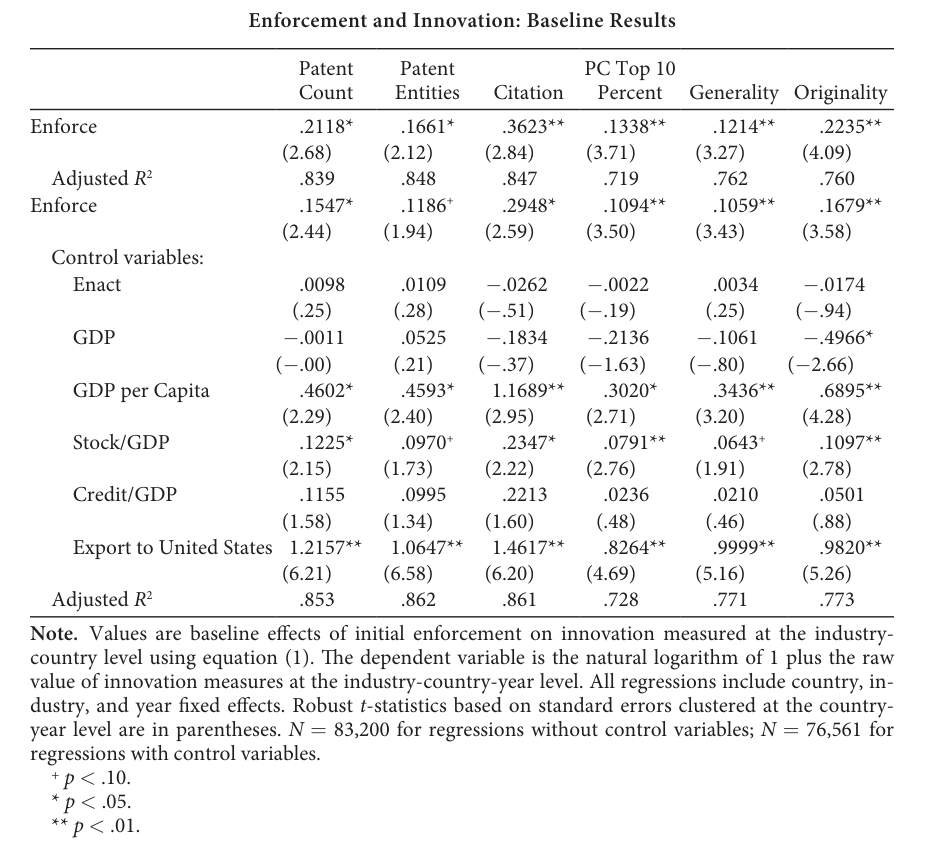
\includegraphics[width = 0.6\textwidth]{tables/baseline_orig}
\end{table}

\subsection{Industry level analysis}\label{subsec:industry-level-analysis}
The authors then proceed to evaluate the problem at industry granularity: they introduce an industry dummy $I_i$ to the baseline regression:
\begin{equation}
    Y_{ict} = \beta_0 + \beta_1 I_i E_{ct} + \lambda X'_{ict} + \delta_{ct} + \delta_{it} + \varepsilon_{ict},
\end{equation}
finding similar results to the baseline regression.

\subsection{Robustness and validation}\label{subsec:robustness-and-validation}
The authors perform various tests and robustness checks, including:
\begin{itemize}
    \item Check for omitted variable bias by including and excluding a large set of additional controls, composed of several indictors of securities-market reforms and policies toward international capital flows; an array of indicators of bank
    regulatory and supervisory policies; and enactment of patent laws, measures of intellectual-property-rights protection, property-rights protection more generally, and the effectiveness of the legal system.
    They find that including or excluding these controls do not alter the results.
    \item Do not find any pretrends in the patent-based measures of innovation before enforcement, based on graphical analysis.
    \item Find that the growth rates in innovation measures do not predict the enforcement of the laws, using a Hazard-Model estimation.
\end{itemize}

\subsection{Dynamic}\label{subsec:dynamic}
The authors study the behaviour of the innovation proxies in a $(-5,10)$ window around the enforcement year, implementing:
\begin{equation}
    Y_{ct}  = \alpha_0 + \sum_{\tau=-5}^{10} \alpha_{1,\tau} E_{c,t,\tau} +\delta_c +\delta_t + \varepsilon_{ct}
\end{equation}
They find a sizeable increase in innovation around the treatment year, while the control variables stay almost constant, as can be seen in figure~\ref{fig:dynamic_orig}.

\begin{figure}[h!]
    \centering
    \begin{subfigure}[b]{0.45\textwidth}
        \centering
        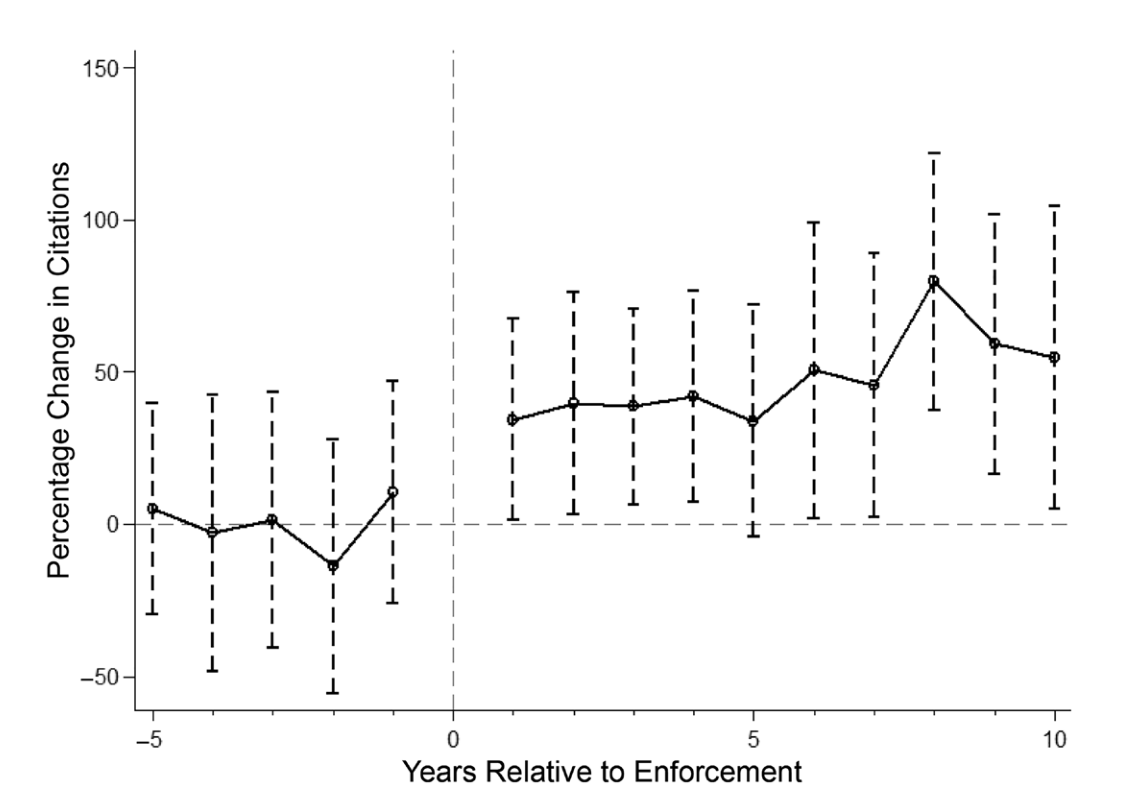
\includegraphics[width=\textwidth]{images/dynamic_orig_citations}
        \caption{Citation Weight}
    \end{subfigure}
    \hfill
    \begin{subfigure}[b]{0.45\textwidth}
        \centering
        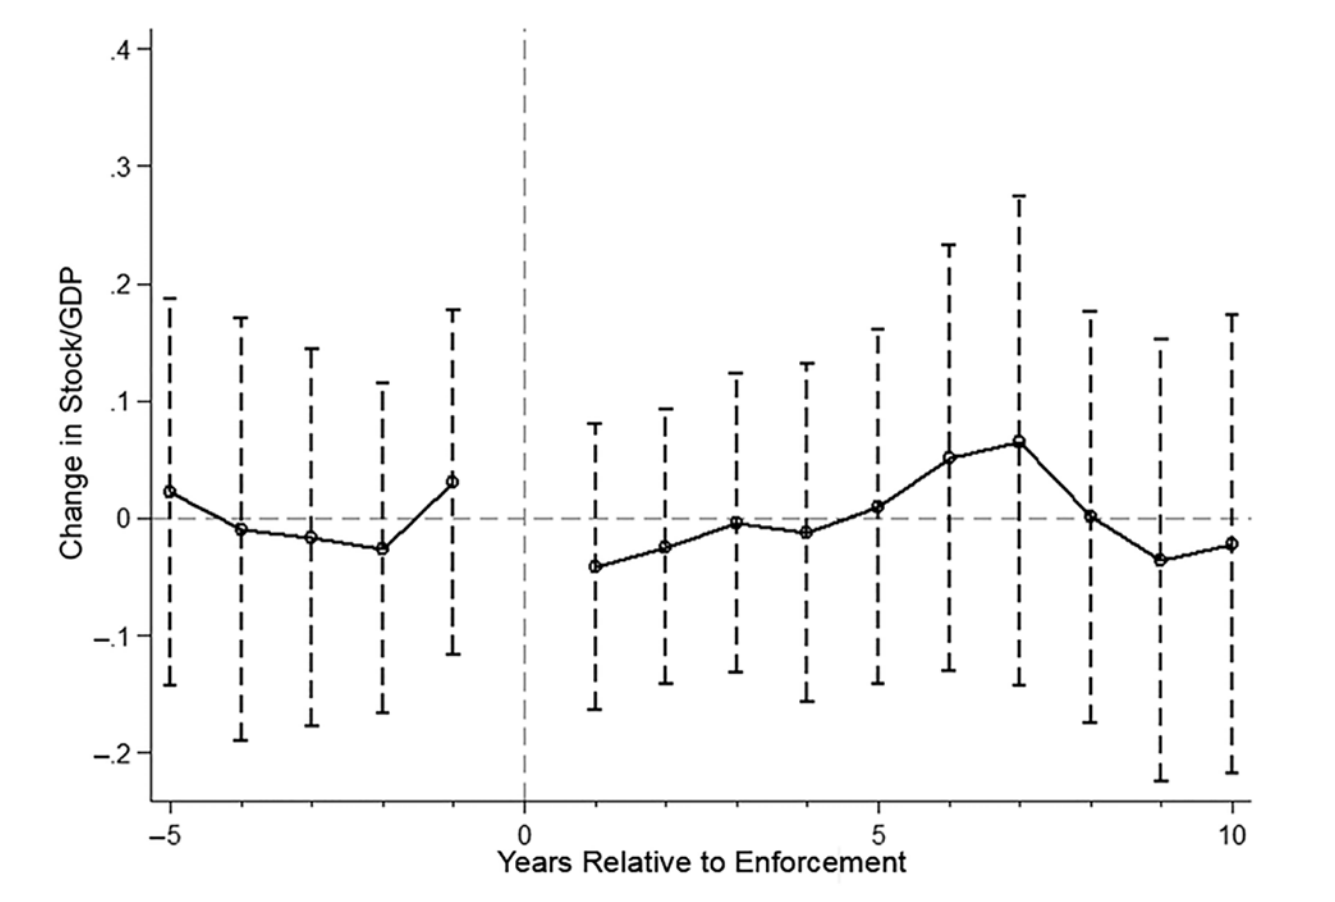
\includegraphics[width=\textwidth]{images/dynamic_orig_stock}
        \caption{Stock Market Capitalization}
    \end{subfigure}

    \vspace{0.5cm}

    \begin{subfigure}[b]{0.45\textwidth}
        \centering
        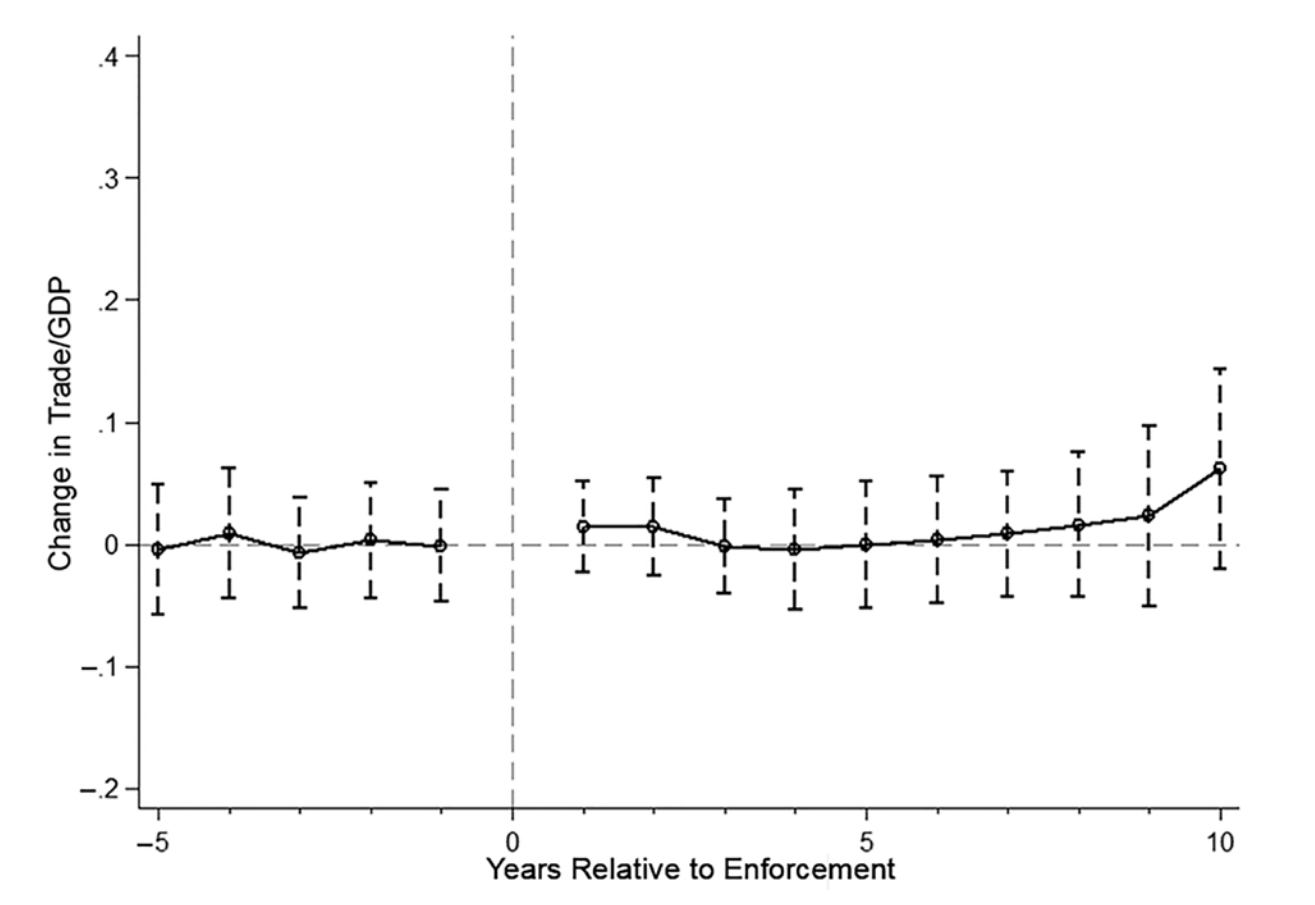
\includegraphics[width=\textwidth]{images/dynamic_orig_trade}
        \caption{Trade}
    \end{subfigure}
    \hfill
    \begin{subfigure}[b]{0.45\textwidth}
        \centering
        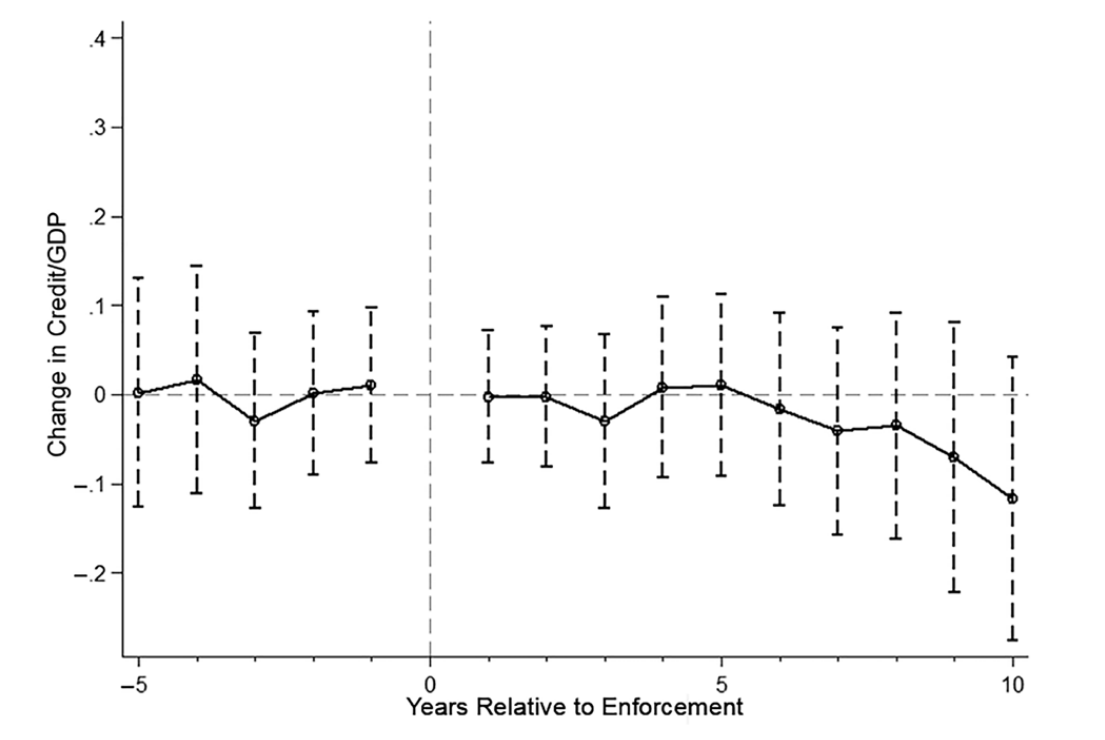
\includegraphics[width=\textwidth]{images/dynamic_orig_credit}
        \caption{Credit}
    \end{subfigure}
    \caption{Dynamic Effects on Citation Weight, Stock Market Capitalization, Trade and Credit}
    \label{fig:dynamic_orig}
\end{figure}